\documentclass[a4paper,11pt]{article}
\usepackage[utf8]{inputenc}
\usepackage[usenames,dvipsnames]{color}
\usepackage{graphicx}
\usepackage[justification=centering,labelfont=bf]{caption}
\usepackage{listings}
\usepackage{minted}
\usepackage[hidelinks]{hyperref}
\begin{document}
\begin{titlepage}
\begin{center}
\textsc{\Large Parallelism}
\\
\texttt{1202}
\\[1.5cm]
\rule{\linewidth}{0.5mm}
\\[0.4cm]
{\huge
\bfseries
Lab 3: Divide and conquer parallelism with OpenMP - Sorting
\\[0.4cm]
}
\rule{\linewidth}{0.5mm}
\\[2.5cm]
\begin{minipage}{0.4\textwidth}
\begin{flushleft}
\large
Héctor Ramón Jiménez
\end{flushleft}
\end{minipage}
\begin{minipage}{0.4\textwidth}
\begin{flushright}
\large
Alvaro Espuña Buxó
\end{flushright}
\end{minipage}
\vfill
{\large
\today
}
\\
{\large
\texttt{Facultat d'Informàtica de Barcelona}
}
\end{center}
\end{titlepage}
\section{Analysis with Tareador}
\begin{enumerate}
\setcounter{enumi}{0}
\item
\textbf{Include the source of the sequential multisort.c code modified
  with the calls to the Tareador API and the task graph generated.}

As we can see in {\tt multisort-tareador.c}, in the {\tt main}
function we only instrumented the call to \texttt{do\_sort} with
randomly generated data because it's the only one we care. To increase
the granularity, and to understand better what's going on with the
recursive calls we also instrumented {\tt multisort} with appropriate
names ({\tt multisort-i}, {\tt merge-n-i}, {\tt basicsort}). We did a
similar thing for merge.

\vspace{0.5cm}
\begin{figure}[h!]
  \center
  \includegraphics[width=1.0\textwidth,trim={2cm 0 0 0},clip]{figs/multisort_tareador.pdf}
  \caption{Detail of the output of tareador for
    multisort-tareador. The full graphic is in
    {\tt multisort\_tareador.pdf}.}
  \label{fig:multisort-tareador}
\end{figure}
\vspace{0.5cm}

From the figure \ref{fig:multisort-tareador} we can see how the {\tt
  basicsort}s are fully parallelizable. The two merges of size n/4 for
every call to {\tt multisort} are also mutually parallelizable. They
only depend on the sorting of the relevant subarray. The call for size n/2 has to wait
for them though.

\item
  \textbf{Write a table with the execution time and speed-up predicted
    by Dimemas (for 1, 2, 4, 8, 16, 32 and 64 processors) for the task
    decomposition specified with Tareador. Are the results close to the
    ideal case? Reason about your answer.}

\begin{figure}[h!]
  \center
\begin{tabular}{| c || c | c |}
\hline
\textbf{N} & \textbf{Time (s)} & \textbf{Speedup}
\\
\hline
\hline
 1 & 53.843 &     - \\ \hline
 2 & 30.379 & 1.772 \\ \hline
 4 & 18.592 & 2.895 \\ \hline
 8 & 12.701 & 4.239 \\ \hline
16 & 10.091 & 5.335 \\ \hline
32 &  8.895 & 6.053 \\ \hline
64 &  8.326 & 6.467 \\ \hline

\end{tabular}
\caption{Table for times and speedup as a function of the number of threads (N)}
\label{fig:speedup-table}
\end{figure}

In figure \ref{fig:speedup-table} we can see that the scalability
degrades past 8 threads. This result is expected since due to
data dependencies, the program is not fully parallelizable (being the
merging the bottleneck). The critical path for mergesort is {\tt
  basicsort} $\rightarrow$ {\tt merge n/4} $\rightarrow$ {\tt merge n/2}. We can see in the
following graphics how the merging is being the bottleneck as we
increase the number of threads (clearly noticeable with 32 threads) while
the {\tt basicsort}ing (in pink) is clearly fully parallelizable.

Probably it is more scalable than reported by Dimemas, because Tareador is
taking into account the initialization of the array, which is sequential.

\vspace{0.5cm}
\begin{figure}[h!]
  \center
  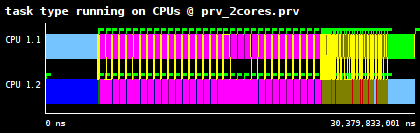
\includegraphics[width=1.0\textwidth]{figs/paraver_2_cores.png}
  \caption{Dimemas simulation with 2 cores}
\end{figure}

\vspace{0.5cm}
\begin{figure}[h!]
  \center
  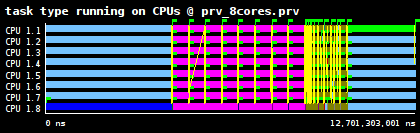
\includegraphics[width=1.0\textwidth]{figs/paraver_8_cores.png}
  \caption{Dimemas simulation with 8 cores}
\end{figure}

\vspace{0.5cm}
\begin{figure}[h!]
  \center
  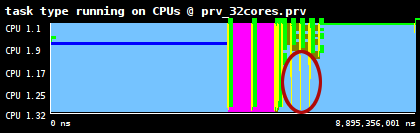
\includegraphics[width=1.0\textwidth]{figs/paraver_32_cores.png}
  \caption{Dimemas simulation with 32 cores. The red \emph{circle} shows how the
    merging doesn't scale well (although basicsorting does)}
\end{figure}

\end{enumerate}

\newpage
\section{Parallelization with OpenMP}
\begin{enumerate}
  \setcounter{enumi}{2}
  \item
    \textbf{Briefly describe the two versions (Leaf and Tree)
      implemented, making references to the source code included in
      the compressed tar file.}

    The idea in both versions is to create tasks and add them to a pool,
    so the threads execute them when they can.

\subsection{Leaf}
The leaf version creates a task for every base case. We need to
take care of the syncronization.

\subsubsection{merge}
We create a task for every {\tt basicmerge}. There's no need of
synchronization at this level, both merges are totally parallelizable.

\begin{minted}{c}
void merge(long n, T left[n], T right[n], T result[n*2],
           long start, long length) {
    if (length < MIN_MERGE_SIZE*2L) {
       // Base case
       #pragma omp task
       basicmerge(n, left, right, result, start, length);
    } else {
       // Recursive decomposition
       merge(n, left, right, result, start, length/2);
       merge(n, left, right, result, start + length/2, length/2);
    }
}
\end{minted}

\subsubsection{multisort}
We create a task for every {\tt basicsort}. Here some synchronization is needed.
First of all, we cannot start merging until we have the four subparts sorted.
But every multisort is completely independent from another. Also, as we saw on figure
\ref{fig:multisort-tareador} the merge of size n/2 depends of the previous merges, thus
we need to wait after them.

\begin{minted}{c}
void multisort(long n, T data[n], T tmp[n]) {
    if (n >= MIN_SORT_SIZE*4L) {
        // Recursive decomposition
        multisort(n/4L, &data[0], &tmp[0]);
        multisort(n/4L, &data[n/4L], &tmp[n/4L]);
        multisort(n/4L, &data[n/2L], &tmp[n/2L]);
        multisort(n/4L, &data[3L*n/4L], &tmp[3L*n/4L]);
        #pragma omp taskwait

        merge(n/4L, &data[0], &data[n/4L], &tmp[0], 0, n/2L);
        merge(n/4L, &data[n/2L], &data[3L*n/4L], &tmp[n/2L], 0, n/2L);
	#pragma omp taskwait

        merge(n/2L, &tmp[0], &tmp[n/2L], &data[0], 0, n);
    } else {
        #pragma omp task
        basicsort(n, data);
    }
}
\end{minted}

\subsection{Tree}

In the tree version, we create a task for every inner node. In this version
two more {\tt taskwaits} are needed.

\subsubsection{merge}
We create a task for every {\tt merge} call. Notice how the {\tt
  taskwait} here is needed, otherwise, two new {\tt merge}s on the
same subpart of the vector could be started.

\begin{minted}{c}
void merge(long n, T left[n], T right[n], T result[n*2],
           long start, long length) {
    if (length < MIN_MERGE_SIZE*2L) {
        // Base case
        basicmerge(n, left, right, result, start, length);
    } else {
        // Recursive decomposition
        #pragma omp task
        merge(n, left, right, result, start, length/2);
	#pragma omp task
        merge(n, left, right, result, start + length/2, length/2);
	#pragma omp taskwait
    }
}
\end{minted}

\subsubsection{multisort}
We create a task for every {\tt multisort} call. When we are finished
sorting, (hence the {\tt taskwait} we can start the merging. Now, we
create a task for every call to {\tt merge} with size n/4. As in the
leaf case, we need to wait both are merged to start the merging with
size n/2. Notice how the taskwait is needed after the last merge. To
understand this, assume 4 divisions (1 multisort call). If 1 is done
and 0 is still going, a merge of 2 could be started (on the
\emph{upper} level), but it could produce an incorrect result.

\begin{minted}{c}
void multisort(long n, T data[n], T tmp[n]) {
    if (n >= MIN_SORT_SIZE*4L) {
        // Recursive decomposition
	#pragma omp task
        multisort(n/4L, &data[0], &tmp[0]);
	#pragma omp task
        multisort(n/4L, &data[n/4L], &tmp[n/4L]);
	#pragma omp task
        multisort(n/4L, &data[n/2L], &tmp[n/2L]);
	#pragma omp task
        multisort(n/4L, &data[3L*n/4L], &tmp[3L*n/4L]);
	#pragma omp taskwait

	#pragma omp task
        merge(n/4L, &data[0], &data[n/4L], &tmp[0], 0, n/2L);
	#pragma omp task
        merge(n/4L, &data[n/2L], &data[3L*n/4L], &tmp[n/2L], 0, n/2L);
	#pragma omp taskwait

        merge(n/2L, &tmp[0], &tmp[n/2L], &data[0], 0, n);
	#pragma omp taskwait
    } else {
        // Base case
	basicsort(n, data);
    }
}
\end{minted}

It's important to note that both versions are probably not technically
optimal.  When we are done with the two first multisorts, we could
start the first merge of size n/4. We avoided this, to benefit from
the simplicity of this code.
\end{enumerate}

\section{Performance analysis}
\textbf{Write a text, inspired in the one provided below, summarizing
  the performance results for the two versions (Leaf and Tree) of
  multisort.}

The performance of the two parallelization strategies for multisort
has been analyzed on a multiprocessor architecture with 12 Intel
cores ... /* complete this paragraph with the information you got in
the first laboratory assignment */.  For all the performance results we
have used an input vector of size XXX randomly generated by the
program itself. The program performs several sort steps in order to
verify the influence of the randomness of the data in the input
vector. The recursive depth of the multisort algorithm is controlled
with /* complete this paragraph with the appropriate information */
The first conclusion of the analysis is that version XXX has better
scalability than version YYY. This is due to the fact that the
parallelism exploited in version YYY is limited by /* complete the
paragraph with an appropriate reasoning */. Figure 1 shows the
execution timelines visualized with Paraver, supporting the previous
argument.  Figure 2 plots the speedup, with respect to the sequential,
for different vector sizes (8, 16 and 32 Megaelements), for the two
OpenMP versions and for the different invocations of multisort in the
main program.

\end{document}
